\documentclass{article}
\usepackage{textcomp}
\usepackage[english]{babel}
\usepackage[utf8]{inputenc}
\usepackage{lmodern}
\usepackage{textcomp}
\usepackage[T1]{fontenc}
\usepackage{ucs}
\usepackage{amssymb}
\usepackage{amsmath}
\usepackage{courier}
\usepackage{graphicx}
\usepackage{a4wide}

\newcommand{\quality}[1]{q_{#1}}
\newcommand{\minfun}{\text{min}}
\newcommand{\realvec}[1]{\mathbf{#1}}
\newcommand{\norm}[1]{\left\| #1 \right\|}
\newcommand{\derivative}[2]{\frac{\partial #1}{\partial #2}}
\newcommand{\timederivative}[1]{\derivative{#1}{t}}
\newcommand{\realnumber}{\mathbb{R}}
\setcounter{secnumdepth}{2}

\author{Jonas Östlund\\jonas@anemomind.com}
\date{\today}
\title{Anemomind Authentication API}

\begin{document}
\maketitle
\section{Introduction}
The part of the software that runs on the server exhibits
an HTTP REST API at \texttt{www.anemolab.com}. To access certain resources
on the server, authentication is required. For this purpose, token-based
authentication is employed.

Token-based authentication can be summarized as follows. When a user who is registered at \texttt{anemolab.com} needs to access a resource on the server, he will need a token. A token is a piece of data that the client, e.g. the web browser, receives from the server when the user logs in. Every time the client needs to request data from the server or modify data, it will send an HTTP request to the server that contains the token. When the server receives the request from the client, it will check that the token provided is one that has been emitted from the server.

The server is implemented in \texttt{node.js} and uses the library \texttt{jwt-simple} to manage tokens. When a registered user requests a token, this request will usually be handled by \texttt{server/auth/local/index.js} which will generate a token for that user by encrypting the user account id using the \texttt{signToken} function located in \texttt{server/auth/auth.service.js}. Then token is returned as a JSON object:
\begin{verbatim}
var token = auth.signToken(user._id, user.role);
res.json({token: token});
\end{verbatim}
Once a registered user has obtained a token, this token will be attached by the client to every subsequent HTTP request made by the client, until the token expires and a new token has to be acquired. Take a look at \texttt{server/api/user/index.js}. This file exhibits an API to access and modify information related to a user. However, in order to protect information related to a user, middlewares from the \texttt{auth} service are inserted before the resource can be accessed. This middleware is defined in \texttt{server/auth/auth.service.js}. A function here is \texttt{isAuthenticated}, which creates a middleware that controls whether or not a token provided in the HTTP request is a valid one.

\begin{verbatim}
if(req.query && req.query.hasOwnProperty('access_token')) {
  req.headers.authorization = 'Bearer ' + req.query.access_token;
}
validateJwt(req, res, next);
\end{verbatim}
In the following sections, we demonstrate how this API can be practically consumed by a client.
\section{Registering a test user}
For testing purposes, we register a new user on the webpage, at \texttt{www.anemolab.com/signup}.
\begin{center}
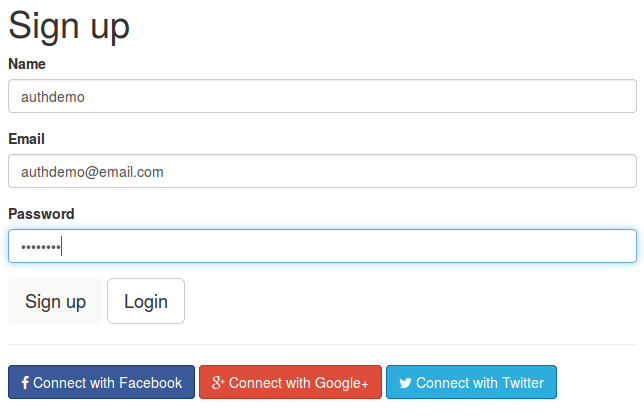
\includegraphics[width=0.5\textwidth]{signup.png}
\end{center}

In this example, the name is \texttt{authdemo}, the e-mail \texttt{authdemo@email.com} and the password \texttt{kalle123}.
\section{Obtaining a token}
Using the registered test user
\section{Accessing data that requires authentication}
\end{document}


